\documentclass[english,inz,shortabstract]{iithesis}

\usepackage[utf8]{inputenc}
\usepackage{natbib}
\usepackage[nottoc,notlot,notlof]{tocbibind}
\usepackage{graphicx}
\usepackage{enumitem}

\newcommand{\oldrovername}{$\aleph_1$\ }
\newcommand{\rovername}{$\aleph_2$\ }

\englishtitle   {Control software for the \fmlinebreak Aleph2 robot - a Mars rover prototype}
\polishtitle    {Oprogramowanie do kontroli robota\fmlinebreak Aleph2 - prototypu łazika marsjańskiego}
\author         {Błażej Sowa}
\advisor        {dr Marek Materzok}
%\date          {}

\englishabstract{
    The \oldrovername (pron. aleph one) robot is a Mars rover prototype being developed since 2015 by the student research group \textit{Continuum}, operating at the University of Wroclaw. One of the team's most outstanding achievements is 2nd place at the \textit{University Rover Challenge 2017}, where the rover proved itself well performing tasks in the desert in Utah.\\
    The thesis focuses on the implementation of the hardware abstraction layer and the simulation environment created for the successor of the aforementioned robot, \rovername (pron. aleph two). The software is largely based on the use of the Robot Operating System (ROS), ros\_control framework and Gazebo simulator.
}

\polishabstract{
    Robot \oldrovername (czyt. alef jeden) to prototyp łazika marsjańskiego rozwijany od 2015 roku przez koło naukowe \textit{Continuum}, działające na Uniwersytecie Wrocławskim. Do jednych z najwybitniejszych osiągnięć drużyny można zaliczyć 2. miejsce na zawodach \textit{University Rover Challenge 2017}, gdzie łazik bardzo dobrze sprawdził się wykonując zadania na pustyni w Utah.\\    
    Praca skupia się na implementacji warstwy abstrakcji sprzętowej oraz środowisku symulacyjnym stworzonych na potrzeby następcy wyżej wspomnianego robota, \rovername (czyt. alef dwa). Oprogramowanie opiera się w znacznym stopniu na wykorzystaniu Robot Operating System (ROS), frameworku ros\_control i symulatora Gazebo. 
}

\begin{document}

\chapter{Introduction}

\section{Background}
The NASA's \textit{Mars Exploration Rover} mission has inspired various annual robotic competitions for university level students that challenge teams to build a robot that would help early explorers on Mars. 
The \textit{Rover Challenge Series} is a series of such competitions run by the \textit{Mars Society}. Among the most popular are \textit{University Rover Challenge} (hosted since 2007) and \textit{European Rover Challenge} (hosted since 2014).

The tasks on the competitions often include:
\begin{itemize}[itemsep=0pt, parsep=2pt, topsep=0pt]
    \item Navigation through rough terrain
    \item Picking up and transporting objects
    \item Flipping switches on the control panel 
    \item Collecting and examining soil samples
    \item Autonomous navigation between predefined points
\end{itemize}

\textit{Continuum} (also known as \textit{Team Continuum} or \textit{Continuum Rover Team}) is a student research club from University of Wroclaw whose main focus is to build and improve its Mars rover prototype and compete in the challenges. The team operates since 2014 and debuted with the \oldrovername (pron. aleph one) robot scoring 3rd place at \textit{University Rover Challenge 2016} and 2nd place at \textit{University Rover Challenge 2017}.

Now, the team is focused on improving the \rovername rover (Fig. \ref{fig:lazik1} and \ref{fig:lazik2}), which is the next iteration of the \oldrovername robot. 


\begin{figure}[h]
    \vspace{0.4cm}
    \hspace*{\fill}
    \begin{minipage}{.45\textwidth}
      \centering
      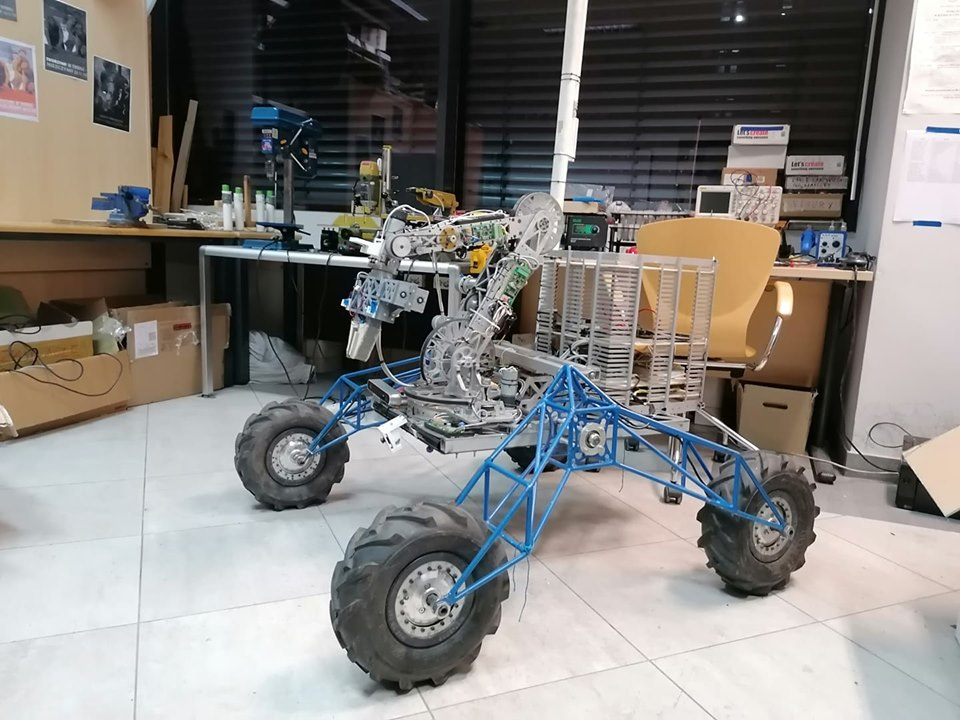
\includegraphics[height=4cm]{img/lazik1.jpg}
      \caption{The current appearance of the \rovername rover}
      \label{fig:lazik1}
    \end{minipage}
    \hfill
    \begin{minipage}{.45\textwidth}
      \centering
      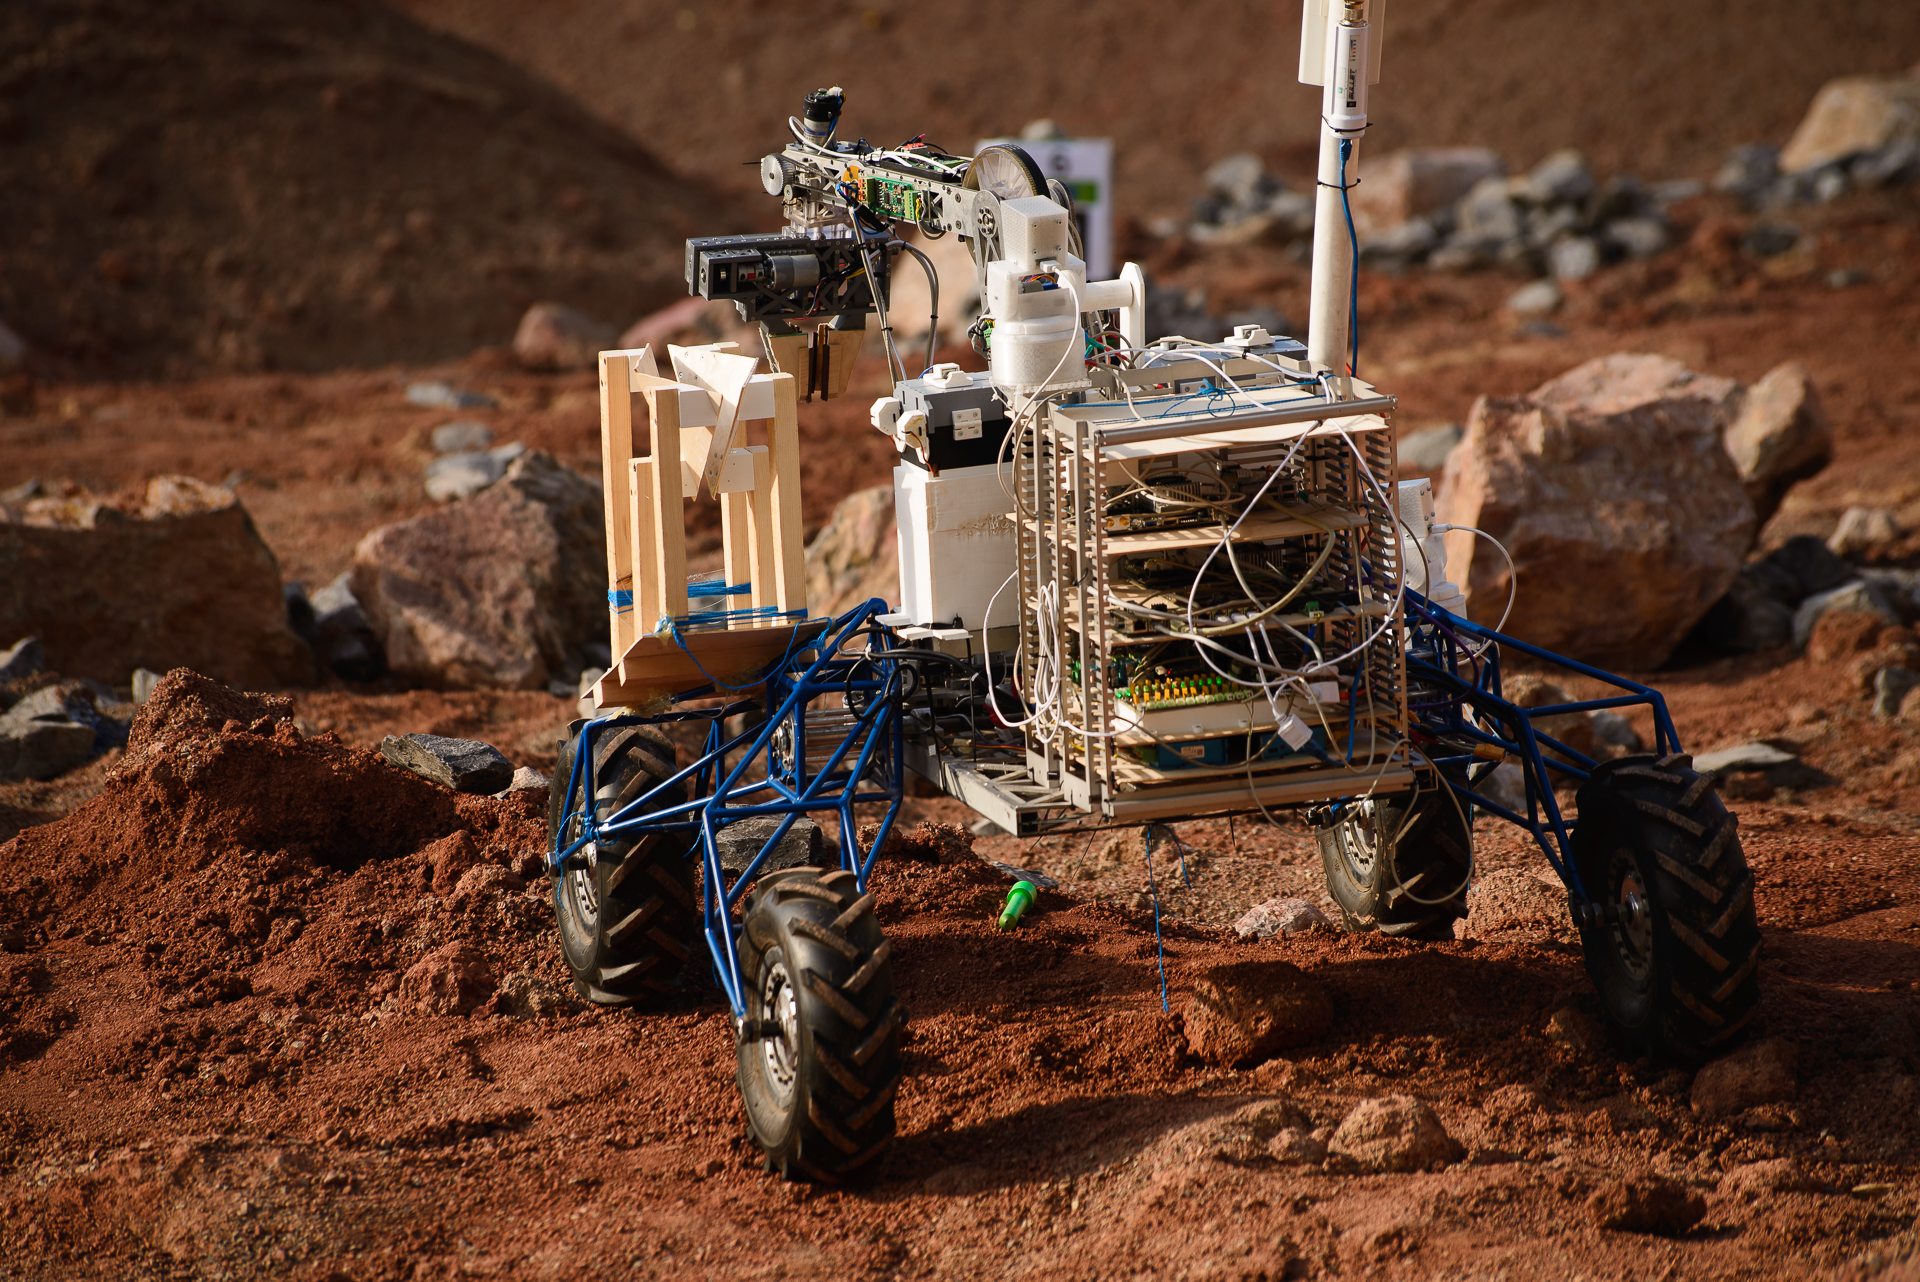
\includegraphics[height=4cm]{img/lazik2.jpg}
      \caption{\rovername performing a task on the \textit{European Rover Challenge 2019}}
      \label{fig:lazik2}
    \end{minipage}
    \hspace*{\fill}
\end{figure}

\section{Motivation}
Although the \oldrovername rover is a well-proven construction piece, its software responsible for robot control and communication with the hardware leaves a lot of room for improvement. The main problems identified are:
\begin{itemize}
    \item \textbf{Unstable implementation} - the software responsible for the drivetrain often fails to communicate with the motor drivers due to only partial implementation of the communication protocol and various race conditions.
    \item \textbf{Hard-coded configuration} - all of the configuration (e.g. IDs of the motor drivers, joint names and limits) is embedded into the source code. This makes it needlessly difficult to reconfigure the programs after making changes to other robot subsystems (hardware or software).
    \item \textbf{Lack of abstraction layers} - the software does not provide any libraries for the implemented controllers or communication protocols. All of these components are placed into single executables. This makes it hard to reuse the code for other purposes.
\end{itemize}
These issues, together with the passion for robots, were the main reasons that led to the decision of making new control software for the \rovername rover.

\section{Goals}
To address the mentioned issues with the previous system, a set of design assumptions that the new software has to meet have been defined. The main assumptions include:

\begin{itemize}
    \item \textbf{Extensive use of open source software} - by relying on widely used and well tested open source projects, the software can be more stable and developed faster.
    \item \textbf{No hard-coded configuration} - the programs should not assume much about the hardware they are running on. Instead, they should read the configuration at runtime. The configuration should be well-documented and easily editable.
    \item \textbf{Hardware abstraction layer} - the software should deliver an abstraction over the hardware it is communicating with by providing interfaces that define its capabilities. This should greatly improve the code reusability. 
    \item \textbf{Simulation environment} - the software should provide the ability to simulate the robot operation in a virtual world. The simulation should be able to run the same set of controllers (ideally, with the same configuration) and provide the same control interfaces as the real robot.
\end{itemize}


\section{Used technologies}

    \subsection{ROS}

    \subsection{ros\_control}

    \subsection{Gazebo}

    \subsection{CANOpen}

    \subsection{RUBI}


\chapter{Documentation of the ROS package stack}

\section{Overview of provided packages}

\section{aleph2\_description}

\section{aleph2\_hardware\_interface}

\section{aleph2\_gazebo}

\section{aleph2\_bringup}

\chapter{Usage}

\chapter{Conclusion}

\bibliographystyle{plain}
\bibliography{bibliography}

\end{document}
